\section{Bridging the Gap: Why Deep Machine Learning Feels Abstract}  

Someone once asked me:

\begin{quote}
\textit{"Hey, you do machine learning, right? What are these weird integrals with $d\mu$ everywhere? Are we still doing calculus or what?"}
\end{quote}

And honestly? I get it.

Modern machine learning papers are filled with expressions like:

\[
\int f \, d\mu
\]

They show up in everything from loss function expectations to probability distributions over infinite-dimensional spaces. And to anyone familiar with classic calculus, this looks like alien notation. What happened to our good old friend \( dx \)?

Well, the short answer is: this isn’t just integration anymore: it’s measure theory. And measure theory is where things start getting... existential. 

\begin{figure}[H]
\centering
\begin{tikzpicture}[every node/.style={font=\footnotesize}]

% Panel 1 — ML student confused
\comicpanel{0}{4}
  {ML Student}
  {Analyst}
  {I just wanted to train a model. Why am I integrating with respect to \textit{mu}?}
  {(-0.6,-0.5)}

% Panel 2 — Analyst explains
\comicpanel{6.5}{4}
  {ML Student}
  {Analyst}
  {Because some functions aren't nice. And Lebesgue integration lets us handle them without crying.}
  {(.6,-0.5)}

% Panel 3 — ML student suspicious
\comicpanel{0}{0}
  {ML Student}
  {Analyst}
  {So this is math therapy for pathological functions?}
  {(-0.8,-0.7)}

% Panel 4 — Analyst shrugs
\comicpanel{6.5}{0}
  {ML Student}
  {Analyst}
  {Pretty much. And your loss function lives here in measure theory land, now. Welcome.}
  {(0.7,-0.6)}

\end{tikzpicture}
\caption{Lebesgue integration: now standard in ML, and... still confusing.}
\end{figure}

So yes—the notation is confusing because what we’re measuring is incredibly abstract. With Riemann integration, everything felt tangible—you could imagine stacking up little rectangles under a curve. But Lebesgue integration operates in a world where we sum values over scattered, fragmented sets. Some of these “sets” barely behave like numbers at all. 

It’s not just a different notation—it’s a different worldview.

To really grasp it, we need to ask:

\begin{quote}
\textbf{What problem was Lebesgue integration trying to solve in the first place?}
\end{quote}

And that’s where it gets interesting. Because mathematics, like machine learning, doesn’t evolve smoothly—it breaks.

\begin{figure}[H]
\centering
\begin{tikzpicture}[every node/.style={font=\footnotesize}]

% Panel 1 — student struggling with abstraction
\comicpanel{0}{4}
  {Student}
  {Lebesgue}
  {I miss Riemann. He let me stack rectangles. You just give me this weird $\int f\, d\mu$ thing.}
  {(-0.6,-0.5)}

% Panel 2 — Lebesgue explains calmly
\comicpanel{6.5}{4}
  {Student}
  {Lebesgue}
  {That's because I’m measuring over messy sets instead of neat intervals. Welcome to the deep end.}
  {(.55,-0.5)}

% Panel 3 — student is clearly panicking
\comicpanel{0}{0}
  {Student}
  {Lebesgue}
  {Wait... some of these “sets” don’t even feel like numbers anymore. Am I still doing math?}
  {(-0.65,-0.6)}

% Panel 4 — Lebesgue smirks
\comicpanel{6.5}{0}
  {Student}
  {Lebesgue}
  {Notation didn’t get weird. Reality did.}
  {(0.75,-0.6)}

\end{tikzpicture}
\caption{Lebesgue integration: it’s not just a different notation; it’s a different universe.}
\end{figure}


\section{How Math Fell Apart, Got Rebuilt, and Accidentally Invented AI}

\subsection{The Calculus Crisis: How Math Broke Down and Rebooted Itself (and Somehow Led to Neural Nets)}

Thomas Kuhn introduced the philosophy of scientific revolutions: progress doesn’t come from small refinements, but from earthquakes that overturn everything that came before. Every time mathematicians thought they had figured it all out, something came along and shattered their understanding, forcing them to rebuild from the ground up.

And today, we’re going to do exactly that one of the biggest breakthroughs in modern analysis. But before you start yawning, let me make a deal with you: like a shady salesman, I promise to make it entertaining.

\begin{itemize}
    \item I’ll throw in \textbf{philosophical crises} (mathematicians panicking).
    \item You’ll get \textbf{plenty of drama} (fights over notation, people possibly getting drowned at sea).
    \item And I’ll even include a bit of \textbf{suspense} (what’s the deal with those weird functions no one could integrate?).
\end{itemize}

But here’s the twist: this isn't just a historical detour. We’re going to connect all of this to something that seems completely unrelated at first: deep machine learning and high frequency trading.  

\begin{figure}[H]
\centering
\begin{tikzpicture}[every node/.style={font=\footnotesize}]

% Panel 1 — Executive wants AI but has no idea what it is
\comicpanel{0}{4}
  {Product Owner}
  {Consultant}
  {We need to do AI. Something with deep learning. Maybe throw in some quantum blockchain.}
  {(-0.6,-0.5)}

% Panel 2 — Consultant nods sagely
\comicpanel{6.5}{4}
  {Product Owner}
  {Consultant}
  {Absolutely. Let's integrate gradient-optimized self-attention into your KPI forecast infrastructure.}
  {(.5,-0.5)}

% Panel 3 — Executive tries to keep up
\comicpanel{0}{0}
  {Product Owner}
  {Consultant}
  {Good. Good. Also, make sure it leverages dynamic epistemic reasoning. For synergy.}
  {(-0.7,-0.7)}

% Panel 4 — Consultant closes the sale
\comicpanel{6.5}{0}
  {Product Owner}
  {Consultant}
  {Of course. We’ll backpropagate your corporate teleology through a neural ontology graph.}
  {(0.7,-0.6)}

\end{tikzpicture}
\caption{Machine learning: from centuries of math anxiety to corporate buzzword nirvana.}
\end{figure}


\subsection{Teaching Myself Lebesgue So You Don’t Have To (But Also You Do)}

That’s right. I’m going to show you how Lebesgue integration --- this thing mathematicians spent centuries freaking out over --- is actually one of the key ideas that makes modern machine learning tick. You might think AI is some kind of black magic, but by the end of this, you’ll see the magician’s tricks. 

Also, I'll be honest; I’m doing this more for myself than for you. After all, teaching is the only true way to learn. So buckle up, because if I have to go down this rabbit hole, I’m dragging you with me.  

\begin{figure}[H]
\centering
\begin{tikzpicture}[every node/.style={font=\footnotesize}]

% Panel 1 — Executive makes the big announcement
\comicpanel{0}{4}
  {Executive}
  {Engineer}
  {Our consultants want to ML our stuff. Can you hadoop our data warehouse for them?}
  {(0,-0.5)}

% Panel 2 — Engineer raises eyebrow
\comicpanel{6.5}{4}
  {Executive}
  {Engineer}
  {You know machine learning is just summing over data, right? Like... really fancy averaging.}
  {(0,-0.5)}

% Panel 3 — Executive blinks in confusion
\comicpanel{0}{0}
  {Executive}
  {Engineer}
  {Wait. You mean it’s not... emergent quantum intuition trained on the blockchain?}
  {(0,0.8)}

% Panel 4 — Engineer delivers the truth
\comicpanel{6.5}{0}
  {Executive}
  {Engineer}
  {Nah. It’s basically calculus. Just weirder sets and more GPU screaming.}
  {(0,0.8)}

\end{tikzpicture}
\caption{Behind the magic of AI? Fancy summing — and a lot of very tired math.}
\end{figure}


\textbf{So let’s start at the beginning—where mathematics was just a dream, and no one even knew numbers could betray them.}
